\section{Requisiti}\label{Requisiti}

Il team \texttt{Agents of S.W.E.} ha classififcato e assegnato i requisiti con un identificativo univoco, secondo quanto definito nel documento \textit{Norme di progetto v3.0.0} nella sezione §2.2.2.1.

\subsection{Requisiti Funzionali}\label{RF}
\begin{center}
\begin{longtable}[c]{|m{.13\textwidth}|m{.47\textwidth}|m{.2\textwidth}|m{.11\textwidth}|}
\hline
\rowcolor{bluelogo}\textbf{\textcolor{white}{ID}} & \textbf{\textcolor{white}{Descrizione}} & \textbf{\textcolor{white}{Obbligatorietà}} & \textbf{\textcolor{white}{Fonti}}\\
\hline \hline
\endhead

ROF1 & L'utente deve poter aggiungere una rete bayesiana al sistema & Obbligatorio & UC1\\
\hline
\rowcolor{grigio}ROF1.1 & Il Sistema deve mettere a disposizione un pulsante per avviare l'operazione di selezione del file, contenente la definizione della rete, da caricare & Obbligatorio & UC1\\
\hline
ROF1.2 & Il Sistema deve consentire all'utente di selezionare un file da caricare & Obbligatorio & UC1\\
\hline
\rowcolor{grigio}ROF1.3 & Il Sistema deve mettere a disposizione dell'utente un bottone per avviare l'operazione di caricamento & Obbligatorio & UC1\\
\hline
ROF1.4 & Il Sistema deve visualizzare un messaggio di errore nel caso l'operazione di caricamento del file non sia andata a buon fine & Obbligatorio & UC1 UC8\\
\hline
\rowcolor{grigio}RFF1.4.1 & Il Sistema deve controllare l'estensione del file caricato, accettando come input solamente file in formato \textit{.JSON} & Opzionale & UC1 UC8\\
\hline
RFF1.4.2 & Il Sistema deve visualizzare un messaggio di errore nel caso in cui la struttura interna del file selezionato sia errata & Opzionale & UC1 UC8\\
\hline
\rowcolor{grigio}ROF1.5 & Il Sistema deve interpretare il file caricato, al fine di costruire la rete bayesiana attraverso la sua definizione & Obbligatorio & UC1\\
\hline
RDF1.6 & Il Sistema deve mantenere in memoria, in caso di riavvio, l'ultima rete bayesiana caricata dall'utente & Desiderabile & Decisione Interna\\
\hline
\rowcolor{grigio}ROF1.7 & L'Utente deve visualizzare un messaggio di notifica di avvenuto caricamento della rete bayesiana da lui selezionata & Obbligatorio & UC30\\
\hline
ROF2 & L'utente deve poter collegare un flusso di dati ad ogni nodo desiderato della rete preesistente & Obbligatorio & UC2\\
\hline
\rowcolor{grigio}ROF2.1 & Il Sistema deve interpretare la rete bayesiana caricata, al fine di estrapolarne i nodi e fornirli all'utente sotto forma di lista & Obbligatorio & UC16\\
\hline
ROF2.1.1 & Il Sistema deve mostrare, per ogni nodo, il nominativo dello stesso & Obbligatorio & UC16\\
\hline
\rowcolor{grigio}ROF2.1.2 & Il Sistema deve mostrare, per ogni nodo, una corrispondente checkbox che identifichi lo stato dello stesso: collegato ad un flusso dati oppure no & Obbligatorio & UC16 UC2\\
\hline
ROF2.5 & Il Sistema deve mettere a disposizione dell'utente le impostazioni necessarie per effettuare correttamente il collegamento desiderato & Obbligatorio & UC2\\
\hline
\rowcolor{grigio}ROF2.5.3 & Il Sistema deve fornire un elenco dei flussi dati disponibili per il collegamento & Obbligatorio & UC2\\
\hline
ROF2.5.3.1 & L'Utente deve poter selezionare un database come sorgente dati & Obbligatorio & UC18\\
\hline
\rowcolor{grigio}ROF2.5.3.2 & Il Sistema deve mettere a disposizione dell'utente un elenco di database disponibili & Obbligatorio & UC18\\
\hline
ROF2.5.3.3 & L'Utente deve visualizzare un messaggio di notifica di avvenuta selezione del database che funge da sorgente dati & Obbligatorio & UC31\\
\hline
\rowcolor{grigio}ROF2.5.3.4 & Il Sistema deve fornire un elenco delle tabelle del database selezionato come sorgente di dati & Obbligatorio & UC2 UC18\\
\hline
ROF2.5.3.5 & L'utente deve poter selezionare la tabella del database desiderata & Obbligatorio & UC2\\
\hline
\rowcolor{grigio}ROF2.5.3.6 & Il Sistema deve aggiornare i flussi dati disponibili per la selezione a seconda della tabella selezionata dall'utente & Obbligatorio & UC2\\
\hline
ROF2.5.4 & L'utente deve poter selezionare il flusso dati desiderato per il collegamento & Obbligatorio & UC2\\
\hline
\rowcolor{grigio}ROF2.5.5 & Il Sistema deve mostrare la lista dei possibili stati del nodo selezionato & Obbligatorio & UC2\\
\hline
ROF2.5.6 & Il Sistema deve mettere a disposizione dell'utente, per ogni stato del nodo, la possibilità di aggiungere una soglia collegata allo stato in questione & Obbligatorio & UC2.4\\
\hline
\rowcolor{grigio}ROF2.5.6.1 & Il Sistema deve mettere a dispozione dell'utente un campo dati che permetta di definire il valore numerico della soglia & Obbligatorio & UC2.4\\
\hline
ROF2.5.6.2 & Il Sistema deve mettere a dispozione dell'utente, un campo dati che permetta di definire se il valore numerico definito per la soglia sia un minimo oppure un massimo & Obbligatorio & UC2.4\\
\hline
\rowcolor{grigio}RDF2.5.6.3 & Il Sistema deve mettere a dispozione dell'utente un campo dati che permetta di definire se la soglia sia critica oppure no & Desiderabile & UC2.4 VER-2019-02-08\\
\hline
ROF2.5.6.4 & Il Sistema deve mettere a disposizione dell'utente un pulsante per aggiungere una soglia ad un determinato stato del nodo. Il click di tale pulsante porterà alla comparsa dei campi dati editabili di cui la soglia è costituita & Obbligatorio & UC2.4 Decisione Interna\\
\hline
\rowcolor{grigio}RDF2.5.6.5 & L'utente deve poter aggiungere molteplici soglie associate allo stesso stato del nodo & Desiderabile & UC2.4 Decisione Interna\\
\hline
ROF2.5.7 & L'utente deve poter editare i campi dati per definire correttamente un livello di soglia al di sotto, o al di sopra del quale la probabilità associata a quel dato stato risulta pari al 100\%, mentre le probabilità associate agli altri stati risultano pari allo 0\% & Obbligatorio & UC2.4\\
\hline
\rowcolor{grigio}ROF2.5.8 & Il Sistema deve mettere a disposizione dell'utente un bottone per confermare le proprie scelte riguardanti il collegamento del singolo nodo & Obbligatorio & UC2\\
\hline
ROF2.5.9 & L'Utente deve visualizzare un messaggio di errore nel caso in cui abbia confermato le proprie scelte riguardanti il collegamento del singolo nodo commettendo alcuni errori & Obbligatorio & UC2 UC14\\
\hline
\rowcolor{grigio}ROF2.5.9.1 & Il Sistema deve verificare che l'utente abbia correttamente selezionato un flusso dati per il collegamento del nodo, negando la conferma del collegamento in caso contrario & Obbligatorio & UC2\\
\hline
ROF2.5.9.2 & Il Sistema deve verificare che l'utente abbia aggiunto almeno una soglia per almeno uno stato del nodo, negando la conferma del collegamento in caso contrario & Obbligatorio & UC2\\
\hline
\rowcolor{grigio}ROF2.5.9.4 & Il Sistema deve verificare che gli insiemi di valori associati ai diversi stati attraverso le soglie, siano tra loro coerenti, negando la conferma del collegamento in caso contrario & Obbligatorio & UC2\\
\hline
ROF2.5.9.5 & L'Utente deve visualizzare un differente messaggio di errore a seconda degli errori commessi in sede di collegamento del nodo & Obbligatorio & UC14\\
\hline
\rowcolor{grigio}ROF2.5.10 & Il Sistema deve aggiornare la lista di checkbox, registrando il nuovo stato di ogni nodo (collegato o meno ad un flusso dati) & Obbligatorio & UC2\\
\hline
ROF2.5.11 & Il Sistema deve mettere a disposizione dell’utente, per ogni stato del nodo, la possibilità di rimuovere una soglia collegata allo stato in questione & Obbligatorio & UC2 \\
\hline
\rowcolor{grigio}ROF2.6 & L'utente deve poter scollegare dal flusso un nodo precedentemente collegato & Obbligatorio & UC19 UC2\\
\hline
ROF2.6.1 & Il Sistema deve mettere a disposizione un pulsante, associato al nodo collegato, per lo scollegamento dello stesso dal flusso dati & Obbligatorio & UC19\\
\hline
\rowcolor{grigio}ROF2.6.2 & Il Sistema deve resettare le impostazioni di collegamento del nodo se l'utente clicca il pulsante di scollegamento & Obbligatorio & UC19 UC2\\
\hline
ROF2.6.3 & Il Sistema deve aggiornare la checkbox associata al nodo scollegato, togliendo la spunta di collegamento & Obbligatorio & UC19 UC16\\
\hline
\rowcolor{grigio}ROF2.6.4 & Il Sistema deve rimuovere il pulsante di scollegamento una volta che il nodo è stato scollegato & Obbligatorio & UC19 UC16\\
\hline
ROF2.7 & L'Utente deve visualizzare un messaggio di notifica di avvenuto collegamento di un nodo al flusso dati & Obbligatorio & UC33\\
\hline
\rowcolor{grigio}ROF3 & L'utente deve poter impostare una politica temporale per il ricalcolo delle probabilità condizionate associate ai nodi della rete bayesiana & Obbligatorio & UC3\\
\hline
ROF3.3 & L'utente deve avere la possibilità di definire una politica temporale & Obbligatorio & UC3\\
\hline
\rowcolor{grigio}ROF3.3.1 & Il Sistema deve mettere a disposizione un pulsante per accedere al pannello di configurazione di una politica temporale & Obbligatorio & UC3\\
\hline
ROF3.3.2 & Il Sistema deve mettere a disposizione dell'utente, un pannello di configurazione contenente i campi dati necessari alla definizione di una politica temporale & Obbligatorio & UC3\\
\hline
\rowcolor{grigio}ROF3.3.2.4 & Il Sistema deve mettere a disposizione dell'utente, un campo dati editabile che permetta di definire il numero di secondi di cui è composta la politica temporale & Obbligatorio & UC3\\
\hline
ROF3.3.2.5 & Il Sistema deve mettere a disposizione dell'utente, un campo dati editabile che permetta di definire il numero di minuti di cui è composta la politica temporale & Obbligatorio & UC3\\
\hline
\rowcolor{grigio}ROF3.3.2.6 & Il Sistema deve mettere a disposizione dell'utente, un campo dati editabile che permetta di definire il numero di ore di cui è composta la politica temporale & Obbligatorio & UC3\\
\hline
ROF3.3.3 & L'utente deve poter editare i campi dati per definire correttamente la politica temporale desiderata & Obbligatorio & UC3\\
\hline
\rowcolor{grigio}ROF3.4 & Il Sistema deve mettere a disposizione dell'utente un bottone per confermare la politica temporale da lui definita & Obbligatorio & UC3\\
\hline
ROF3.5 & Il Sistema deve visualizzare un messaggio di errore, contente gli errori commessi, nel caso in cui l'utente abbia confermato una politica temporale non correttamente definita & Obbligatorio & UC15\\
\hline
\rowcolor{grigio}ROF3.5.1 & Il Sistema deve negare la creazione della politica temporale nel caso in cui l'utente abbia confermato una politica temporale non correttamente definita & Obbligatorio & UC3 UC15 \\
\hline
ROF3.5.2 & Il Sistema deve verificare che l'utente abbia editato almeno uno dei tre campi dati, sengalando altrimenti l'errore & Obbligatorio & UC3 UC15\\
\hline
\rowcolor{grigio}ROF3.5.3 & Il Sistema deve verificare che il contenuto del campo dati "secondi" sia un numero intero compreso tra 0 e 59, segnalando altrimenti l'errore & Obbligatorio & UC3 UC15\\
\hline
ROF3.5.4 & Il Sistema deve verificare che il contenuto del campo dati "minuti" sia un numero intero compreso tra 0 e 59, segnalando altrimenti l'errore & Obbligatorio & UC3 UC15\\
\hline
\rowcolor{grigio}ROF3.5.5 & Il Sistema deve verificare che il contenuto del campo dati "ore" sia un numero intero >= 0 & Obbligatorio & UC3 UC15\\
\hline
ROF3.6 & L'Utente deve visualizzare un messaggio di notifica di avvenuta selezione della politica temporale per il ricalcolo delle probabilità & Obbligatorio & UC32\\
\hline
\rowcolor{grigio}ROF4 & Il Sistema deve fornire i dati di monitoraggio relativi ai nodi della rete bayesiana non collegati al flusso & Obbligatorio & UC4 UC20\\
\hline
ROF4.4 & Il Sistema deve mettere a disposizione dell'utente un pulsante per avviare il monitoraggio dei dati & Obbligatorio & UC20\\
\hline
\rowcolor{grigio}ROF4.4.3 & Il Sistema deve visualizzare un messaggio di errore, nel caso in cui l'utente abbia avviato il monitoraggio senza aver preventivamente impostato la politica temporale per il ricalcolo delle probabilità & Obbligatorio & UC20 UC12\\
\hline
ROF4.4.4 & Il Sistema deve visualizzare un messaggio di errore, nel caso in cui l'utente abbia avviato il monitoraggio senza aver preventivamente collegato almeno un nodo della rete bayesiana al flusso dati & Obbligatorio & UC20 UC9\\
\hline
\rowcolor{grigio}ROF4.4.5 & Il Sistema deve memorizzare sul server la rete bayesiana, insieme alle corrispondenti impostazioni di collegamento & Obbligatorio & UC20\\
\hline
ROF4.4.6 & Il Sistema deve impedire all'utente la modifica delle impostazione di collegamento di una rete in fase di monitoraggio & Obbligatorio & UC20\\
\hline
\rowcolor{grigio}RFF4.4.7 & L'Utente deve aver la possibilità di monitorare contemporaneamente più reti bayesiane & Opzionale & Capitolato\\
\hline
RFF4.4.7.1 & Il Sistema deve consentire l'avvio del monitoraggio di una rete anche nel caso in cui vi siano altri monitoraggi attivi & Opzionale & UC20 Capitolato\\
\hline
\rowcolor{grigio}ROF4.4.8 & L'Utente deve visualizzare un messaggio di notifica di avvio del monitoraggio della rete bayesiana, attualmente visualizzata nel pannello & Obbligatorio & UC34\\
\hline
ROF4.5 & Il Sistema deve fornire all'utente una lista di probabilità dinamiche associate ai nodi della rete in monitoraggio & Obbligatorio & UC4\\
\hline
\rowcolor{grigio}RFF4.5.1 & L'Utente deve aver la possibilità di scegliere la rete bayesiana, tra quelle al momento in monitoraggio, di cui visualizzare i dati di monitoraggio sotto forma di probabilità dinamiche & Opzionale & UC4\\
\hline
RFF4.5.1.1 & Il Sistema deve fornire all'utente un menù a tendina contente la lista delle reti bayesiane in monitoraggio tra cui scegliere & Opzionale & UC4\\
\hline
\rowcolor{grigio}ROF4.6 & Il Sistema, attraverso l'uso del server per l'elaborazione dei dati, deve aggiornare periodicamente le probabilità in base a quanto definito come politica temporale per il ricalcolo delle probabilità & Obbligatorio & UC4\\
\hline
RDF4.6.1 & Il Sistema, indipendentemente dalla politica temporale stabilita dall'utente, deve ricalcolare le probabilità al verificarsi del superamento di una soglia critica associata ad uno stato di un nodo collegato al flusso di monitoraggio & Desiderabile & UC4 VER-2019-02-08\\
\hline
\rowcolor{grigio}ROF4.7 & L'Utente deve poter interrompere monitoraggio relativo alla rete correntemente visualizzata nel pannello & Obbligatorio & UC21\\
\hline
ROF4.7.1 & Il Sistema deve mettere a disposizione un pulsante per interrompere il monitoraggio della rete bayesiana & Obbligatorio & UC21\\
\hline
\rowcolor{grigio}ROF4.7.2 & L'Utente deve visualizzare un messaggio di notifica di interruzione del monitoraggio della rete bayesiana attualemnte visualizzata nel pannello & Obbligatorio & UC35\\
\hline
ROF7 & L'Utente deve poter collegare il plug-in al server per l'elaborazione dati e il salvataggio delle impostazioni di collegamento & Obbligatorio & UC17\\
\hline
\rowcolor{grigio}ROF7.1 & Il Sistema deve disporre di una sezione adibita alle "Server Settings" all'interno del menù "Edit" del pannello & Obbligatorio & UC17\\
\hline
ROF7.1.1 & Il Sistema deve disporre di, nella sezione "Server Settings" del menù "Edit" del pannello, un campo di testo in cui inserire l'indirizzo IP del server al quale ci si desidera connettere & Obbligatorio & UC17\\
\hline
\rowcolor{grigio}ROF7.1.2 & Il Sistema deve disporre di, nella sezione "Server Settings" del menù "Edit" del pannello, un campo di testo in cui inserire la porta del server alla quale ci si desidera connettere & Obbligatorio & UC17\\
\hline
ROF7.1.3 & Il Sistema deve disporre di, nella sezione "Server Settings" del menù "Edit" del pannello, un pulsante che permette di confermare i dati inseriti & Obbligatorio & UC17\\
\hline
\rowcolor{grigio}ROF7.2 & L'Utente deve visualizzare un messaggio di errore nel caso in cui il collegamento al server non sia giunto a buon fine& Obbligatorio & UC22\\
\hline
ROF7.2.1 & Il Sistema deve verificare che l'indirizzo IP inserito dall'utente sia valido & Obbligatorio & UC17 UC22\\
\hline
\rowcolor{grigio}ROF7.2.2 & Il Sistema deve verificare che la porta del server indicata dall'utente sia in ascolto & Obbligatorio & UC17 UC22\\
\hline
ROF7.3 & L'Utente deve visualizzare un messaggio di avvenuto collegamento al server, nel caso in cui sia giunto a buon fine & Obbligatorio & UC26\\
\hline
\rowcolor{grigio}RDF8 & L'Utente deve poter selezionare una rete bayesiana, con eventuali relative impostazioni di collegamento, tra quelle precedentemente caricate & Desiderabile & UC23\\
\hline
RDF8.1 & Il Sistema deve mettere a disposizione dell'utente la lista delle reti bayesiane, visualizzate sotto forma di un menù a tendina, salvate nel server & Desiderabile & UC23\\
\hline
\rowcolor{grigio}RDF8.2 & Il Sistema deve mettere a disposizione dell'utente un pulsante per la selezione della rete bayesiana selezionata attraverso il menù a tendina & Desiderabile & UC23\\
\hline
RDF8.3 & Il Sistema, prima di cambiare il contesto di visualizzazione sostituendo le vecchie impostazioni con le nuove, deve salvare nel server la rete precedentemente visualizzata e le sue eventuali impostazioni di collegamento & Desiderabile & UC23\\
\hline
\rowcolor{grigio}RDF8.3.1 & Il Sistema, nel caso in cui la rete da memorizzare sia già presente nel server, deve sovrascrivere le impostazioni di collegamento memorizzate & Desiderabile & UC23\\
\hline
RDF8.3.2 & Il Sistema, nel caso in cui la rete visualizzata prima del cambio di contesto sia attualmente in monitoraggio, non deve effettuare operazioni di memorizzazione su server & Desiderabile & UC23\\
\hline
\rowcolor{grigio}RDF8.4 & Il Sistema, a seguito della scelta dell'utente, deve visualizzare la rete selezionata e le sue relative impostazioni di collegamento che vanno a sostituire quelle precedentemente visualizzate & Desiderabile & UC23\\
\hline
ROF9 & Il Sistema deve mettere a disposizione dell'utente una sezione unicamente dedicata alla visualizzazione dei dati di monitoraggio & Obbligatorio & Decisione Interna UC24\\
\hline
\rowcolor{grigio}ROF9.1 & Il Sistema deve mettere a disposizione un bottone che consenta all'utente di passare alla sezione per la visualizzazione dei monitoraggi attivi & Obbligatorio & UC24\\
\hline
ROF9.1.1 & Il Sistema deve sostituire la precedente vista del pannello e sostituirla con la sezione dedicata alla visualizzazione dei monitoraggi attivi & Obbligatorio & UC24\\
\hline
\rowcolor{grigio}ROF9.2 & Il Sistema deve mettere a disposizione un bottone che consenta all'utente di uscire dalla sezione di visualizzazione dei monitoraggi attivi per tornare alle impostazioni di collegamento  & Obbligatorio & UC25\\
\hline
RDF10 & L'Utente deve poter rimuovere una delle reti memorizzate nel sistema & Desiderabile & UC27\\
\hline
\rowcolor{grigio}RDF10.1 & Il Sistema deve mettere a disposizione un pulsante per l'eliminazione della rete bayesiana selezionata attraverso il menù a tendina & Desiderabile & UC27\\
\hline
RDF10.2 & L'Utente deve visualizzare un messaggio di errore nel caso in cui abbia tentato di rimuovere una rete bayesiana in fase di monitoraggio attivo & Desiderabile & UC28\\
\hline
\rowcolor{grigio}RDF10.2.1 & Il Sistema deve verificare che l'utente non abbia selezionato una rete bayesiana in fase di monitoraggio attivo per la rimozione, bloccando l'operazione in caso contrario & Desiderabile & UC28 UC20\\
\hline
RDF10.3 & Il Sistema deve rimuovere dal server la rete bayesiana, e le relative impostazioni di collegamento, selezionata dall'utente & Desiderabile & UC27\\
\hline
\rowcolor{grigio}RDF10.4 & L'Utente deve visualizzare un messaggio di avvenuta rimozione della rete bayesiana nel caso in cui l'operazione sia andata a buon fine & Desiderabile & UC29\\
\hline
\caption{Requisiti Funzionali}
\end{longtable}
\end{center}


%\subsection{Requisiti Prestazionali}\label{RP}
\subsection{Requisiti di Qualità}\label{RQ}
\begin{center}
\begin{longtable}[c]{|m{.09\textwidth}|m{.48\textwidth}|m{.2\textwidth}|m{.12\textwidth}|}
\hline
\rowcolor{bluelogo}\textbf{\textcolor{white}{ID}} & \textbf{\textcolor{white}{Descrizione}} & \textbf{\textcolor{white}{Obbligatorietà}} & \textbf{\textcolor{white}{Fonti}}\\
\hline \hline
\endhead

ROQ1 & È necessario fornire un manuale utente, per l'utilizzo del prodotto, in formato \textit{pdf} & Obbligatorio & Capitolato\\
\hline
\rowcolor{grigio}ROQ1.1 & Il manuale utente deve essere disponibile in lingua italiana & Obbligatorio & Decisione Interna\\
\hline
RDQ1.2 & Il manuale utente deve essere disponibile in lingua inglese & Desiderabile & Decisione Interna\\
\hline
\rowcolor{grigio}RDQ1.3 & Il manuale utente deve contenere una sezione in cui vengono descritti i possibili errori e malfunzionamenti dell’applicazione & Desiderabile & Decisione Interna\\
\hline
ROQ2 & È necessario fornire un manuale per la manutenzione ed estensione del prodotto & Obbligatorio & Capitolato\\
\hline
\rowcolor{grigio}ROQ2.1 & Il manuale di manutenzione/estensione deve essere disponibile in lingua italiana & Obbligatorio & Decisione Interna\\
\hline
RDQ2.2 & Il manuale di manutenzione/estensione deve essere disponibile in lingua inglese & Desiderabile & Decisione Interna\\
\hline
\rowcolor{grigio}ROQ3 & Il prodotto deve essere sviluppato in modo concorde a quanto stabilito nelle \textit{Norme di Progetto v3.0.0} & Obbligatorio & Decisione Interna\\
\hline
RDQ5 & Il codice sorgente del plug-in deve essere reperibile in una repository pubblica su \textit{GitHub}\glossario o su altre piattaforme di condivisione & Desiderabile & Capitolato \\
\hline
\rowcolor{grigio}RDQ6 & Il plug-in deve essere pubblicato nella sezione plug-in di \textit{Grafana}, disponibile all'indirizzo \url{https://grafana.com/plugins}   & Desiderabile & Decisione Interna \\
\hline
RDQ7 & Il plug-in deve essere compatibile con la versione 6.0.0 di \textit{Grafana}, pubblicata in data 2019-02-25  & Desiderabile & Decisione Interna\\
\hline
\rowcolor{grigio}RDQ8 & La struttura della directory del plug-in deve essere conforme con quanto indicato dalla documentazione di \textit{Grafana}, al link: \url{http://docs.grafana.org/plugins/developing/plugin-review-guidelines/}  & Desiderabile & Decisione Interna \\
\hline
RDQ9 & Deve essere consegnato il Bug Reporting per il tracciamento di tutte le problematiche o anomalie del sistema & Desiderabile & Decisione Interna\\
\hline
\rowcolor{grigio}RDQ10 & La progettazione e la codifica devono rispettare le metriche definite nei documento Piano di Qualifica v3.0.0 & Desiderabile & Decisione Interna\\
\hline
RDQ11 & Lo sviluppo dell'applicativo deve comprendere l'implementazione di test di unità e di intergrazione & Desiderabile & Decisione Interna \\
\hline
\caption{Requisiti di Qualità}
\end{longtable}
\end{center}

\pagebreak

\subsection{Requisiti di Vincolo}\label{RV}
\begin{center}
\begin{longtable}[c]{|m{.1\textwidth}|m{.53\textwidth}|m{.25\textwidth}|}
\hline
\rowcolor{bluelogo}\textbf{\textcolor{white}{ID}} & \textbf{\textcolor{white}{Descrizione}} & \textbf{\textcolor{white}{Fonti}}\\
\hline \hline
\endhead
ROV1 & Il plug-in deve essere sviluppato in linguaggio \textit{ECMAScript6} & \textit{Grafana}: guida per gli sviluppatori.\\
\hline
\rowcolor{grigio}ROV2 & Il punto di ingresso per il plug-in deve essere sviluppato nel file "module.js" & \textit{Grafana}: guida per gli sviluppatori\\
\hline
ROV3 & Va utilizzato un qualsiasi build system\glossario che supporti \textit{systemjs}\glossario & \textit{Grafana}: guida per gli sviluppatori\\
\hline
\rowcolor{grigio}ROV4 & Il codice sorgente del plug-in deve essere open source & Capitolato\\
\hline
ROV5 & La rete bayesiana è definita in un file formato \textit{.JSON} & Capitolato\\
\hline
\rowcolor{grigio}ROV6 & L'interfaccia grafica del plug-in è sviluppata utilizzando \textit{HTML5}\glossario, \textit{CSS3}\glossario e \textit{Angularjs}\glossario & \textit{Grafana}: guida per gli sviluppatori \\
\hline
ROV8 & Il Sistema deve funzionare sul browser \textit{Chrome} dalla versione 58 & \hyperref[SupportoECMAScript]{Supporto al linguaggio ECMAScript6 (§\ref*{SupportoECMAScript})}\\
\hline
\rowcolor{grigio}ROV9 & Il Sistema deve funzionare sul browser \textit{Microsoft Edge} dalla versione 14 & \hyperref[SupportoECMAScript]{Supporto al linguaggio ECMAScript6 (§\ref*{SupportoECMAScript})}\\
\hline
ROV10 & Il Sistema deve funzionare sul browser \textit{Firefox} dalla versione 54 & \hyperref[SupportoECMAScript]{Supporto al linguaggio ECMAScript6 (§\ref*{SupportoECMAScript})}\\
\hline
\rowcolor{grigio}ROV11 & Il Sistema deve funzionare sul browser \textit{Safari} dalla versione 10 & \hyperref[SupportoECMAScript]{Supporto al linguaggio ECMAScript6 (§\ref*{SupportoECMAScript})}\\
\hline
ROV12 & Il plug-in deve funzionare per l'ultima versione di \textit{Grafana} disponibile in tempo di ingresso ad RR: v5.4.3 & Decisione Interna\\
\hline
\caption{Requisiti di Vincolo}
\end{longtable}
\end{center}

\begin{figure}[H]
	\begin{center}
		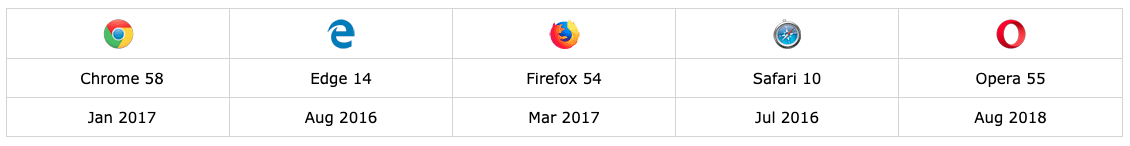
\includegraphics[scale=0.4]{./images/ES6_Support.png}
		 \caption{Supporto al Linguaggio ECMAScript6. Immagine da: \url{https://www.w3schools.com/js/js_es6.asp}}
		 \label{SupportoECMAScript}
	\end{center}
\end{figure}

\pagebreak

%\footnote{Il supporto al linguaggio ECMASCript 6 è il seguente:\\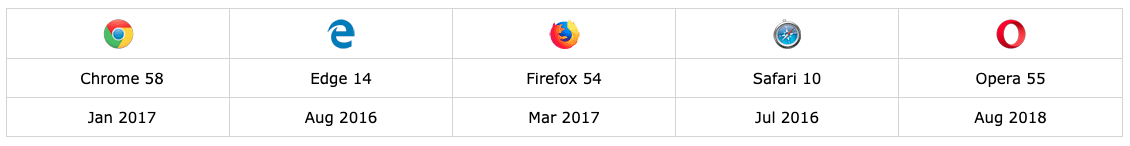
\includegraphics[scale=0.3]{./images/ES6_Support.png}\\Immagine da: \url{https://www.w3schools.com/js/js_es6.asp}}

\subsection{Tacciamento Fonti-Requisiti}\label{Tracciamento}
\begin{center}
\begin{longtable}[c]{|c|m{.15\textwidth}|}
\hline
\rowcolor{bluelogo}\textbf{\textcolor{white}{Fonte}} & \textbf{\textcolor{white}{Requisiti}}\\
\hline \hline
\endhead
Capitolato & \makecell{RFF4.4.7\\RFF4.4.7.1\\ROQ1\\ROQ2\\RDQ5\\ROV4\\ROV6}\\
\hline
\rowcolor{grigio}Decisione Interna & \makecell{ROQ1.1\\RDQ1.2 \\ RDQ1.3\\ROQ2.1\\RDQ2.2\\ROQ3\\RDQ6\\RDF1.6\\RDQ7\\RDQ8 \\ RDQ9 \\ RDQ10 \\ RDQ11\\ROV12\\ROF2.5.6.4\\RDF2.5.6.5\\ROF9}\\
\hline
Piattaforma \textit{Grafana} & \makecell{ROV1\\ROV2\\ROV3\\ROV6}\\
\hline
\rowcolor{grigio}UC1 & \makecell{ROF1\\ROF1.1\\ROF1.2\\ROF1.3\\ROF1.4\\RFF1.4.1\\RFF1.4.2\\ROF1.5}\\
\hline
UC2 & \makecell{ROF2\\ROF2.1.2\\ROF2.5\\ROF2.5.3\\ROF2.5.3.4\\ROF2.5.3.5\\ROF2.5.3.6\\ROF2.5.4\\ROF2.5.5\\ROF2.5.8\\ROF2.5.9\\ROF2.5.9.1\\ROF2.5.9.2\\ROF2.5.9.4\\ROF2.5.10\\ ROF2.5.11\\ROF2.6\\ROF2.6.2}\\
\hline
\rowcolor{grigio}UC2.4 & \makecell{ROF2.5.6\\ROF2.5.6.1\\ROF2.5.6.2\\RDF2.5.6.3\\ROF2.5.6.4\\RDF2.5.6.5\\ROF2.5.7}\\
\hline
UC3 & \makecell{ROF3\\ROF3.3\\ROF3.3.1\\ROF3.3.2\\ROF3.3.2.4\\ROF3.3.2.5\\ROF3.3.2.6\\ROF3.3.3\\ROF3.4\\ ROF3.5.1\\ROF3.5.2\\ROF3.5.3\\ROF3.5.4\\ROF3.5.5}\\
\hline
\rowcolor{grigio}UC4 & \makecell{ROF4\\ROF4.5\\RFF4.5.1\\RFF4.5.1.1\\ROF4.6\\RDF4.6.1}\\
\hline
UC8 & \makecell{ROF1.4\\RFF1.4.1\\RFF1.4.2}\\
\hline
\rowcolor{grigio}UC9 & \makecell{ROF4.4.4}\\
\hline
UC12 & \makecell{ROF4.5.3}\\
\hline
\rowcolor{grigio}UC14 & \makecell{ROF2.5.9\\ROF2.5.9.5}\\
\hline
UC15 & \makecell{ROF3.5 \\ ROF3.5.1\\ROF3.5.2\\ROF3.5.3\\ROF3.5.4\\ROF3.5.5}\\
\hline
\rowcolor{grigio}UC16 & \makecell{ROF2.1\\ROF2.1.1\\ROF2.1.2\\ROF2.6.3\\ROF2.6.4}\\
\hline
UC17 & \makecell{ROF7\\ROF7.1\\ROF7.1.1\\ROF7.1.2\\ROF7.1.3\\ROF7.2\\ROF7.2.1\\ROF7.2.2\\ROF7.3}\\
\hline
\rowcolor{grigio}UC18 & \makecell{ROF2.5.3.1\\ROF2.5.3.2\\ROF2.5.3.4}\\
\hline
UC19 & \makecell{ROF2.6\\ROF2.6.1\\ROF2.6.2\\ROF2.6.3\\ROF2.6.4}\\
\hline
\rowcolor{grigio}UC20 & \makecell{ROF4\\ROF4.4\\ROF4.4.3\\ROF4.4.4\\ROF4.4.5\\ROF4.4.6\\RFF4.4.7.1\\RDF10.2.1}\\
\hline
UC21 & \makecell{ROF4.7\\ROF4.7.2}\\
\hline
\rowcolor{grigio}UC22 & \makecell{ROF7.2\\ROF7.2.1\\ROF7.2.2}\\
\hline
UC23 & \makecell{RDF8\\RDF8.1\\RDF8.2\\RDF8.3\\RDF8.3.1\\RDF8.3.2\\RDF8.4}\\
\hline
\rowcolor{grigio}UC24 & \makecell{ROF9\\ROF9.1\\ROF9.1.1}\\
\hline
UC25 & \makecell{ROF9.2}\\
\hline
\rowcolor{grigio}UC26 & \makecell{ROF7.3}\\
\hline
UC27 & \makecell{RDF10\\RDF10.1\\RDF10.3}\\
\hline
\rowcolor{grigio}UC28 & \makecell{RDF10.2\\RDF10.2.1}\\
\hline
UC29 & \makecell{RDF10.4}\\
\hline
\rowcolor{grigio}UC30 & \makecell{ROF1.7}\\
\hline
UC31 & \makecell{ROF2.5.3.3}\\
\hline
\rowcolor{grigio}UC32 & \makecell{ROF3.6}\\
\hline
UC33 & \makecell{ROF2.7}\\
\hline
\rowcolor{grigio}UC34 & \makecell{ROF4.4.8}\\
\hline
UC35 & \makecell{ROF4.7.2}\\
\hline
\rowcolor{grigio}VER-2019-02-08 & \makecell{RDF4.6.1\\RDF2.5.6.3}\\
\hline
Supporto a \textit{ECMAScript6} & \makecell{ROV8\\ROV9\\ROV10\\ROV11}\\
\hline
\caption{Tracciamento Fonti-Requisiti}
\end{longtable}
\end{center}




\subsection{Tracciamento Requisiti-Fonti}\label{TracciamentoRF}
\begin{center}
\begin{longtable}[c]{|c|m{.30\textwidth}|}
\hline
\rowcolor{bluelogo}\textbf{\textcolor{white}{Requisito}} & \textbf{\textcolor{white}{Fonte}}\\
\hline \hline
\endhead
ROF1 & UC1 \\
\hline
\rowcolor{grigio}ROF1.1 & UC1 \\
\hline
ROF 1.2 & UC1 \\
\hline
\rowcolor{grigio}ROF 1.3 & UC1 \\
\hline
ROF 1.4 & UC1,UC8 \\
\hline
\rowcolor{grigio}ROF 1.4.1 & UC1,UC8 \\
\hline
RFF 1.4.2 & UC1,UC8 \\
\hline
\rowcolor{grigio}ROF 1.5 & UC1 \\
\hline
RDF 1.6 & Decisione Interna \\
\hline
\rowcolor{grigio}ROF 1.7 & UC30 \\
\hline
ROF 2 & UC2 \\
\hline
\rowcolor{grigio}ROF 2.1 & UC16 \\
\hline
ROF 2.1.1 & UC16 \\
\hline
\rowcolor{grigio}ROF 2.1.2 & UC16,UC2 \\
\hline
ROF 2.5 & UC2 \\
\hline
\rowcolor{grigio}ROF 2.5.3 & UC2 \\
\hline
ROF 2.5.3.1 & UC18 \\
\hline
\rowcolor{grigio}ROF 2.5.3.2 & UC18 \\
\hline
ROF 2.5.3.3 & UC31 \\
\hline
\rowcolor{grigio}ROF 2.5.3.4 & UC2,UC18 \\
\hline
ROF 2.5.3.5 & UC2 \\
\hline
\rowcolor{grigio}ROF 2.5.3.6 & UC2 \\
\hline
ROF 2.5.4 & UC2 \\
\hline
\rowcolor{grigio}ROF 2.5.5 & UC2 \\
\hline
ROF 2.5.6 & UC2.4 \\
\hline
\rowcolor{grigio}ROF 2.5.6.1 & UC2.4 \\
\hline
ROF 2.5.6.2 & UC2.4 \\
\hline
\rowcolor{grigio}RDF 2.5.6.3 & UC2.4,VER-2019-02-08 \\
\hline
ROF 2.5.6.4 & UC2.4,Decisione Interna \\
\hline
\rowcolor{grigio}RDF 2.5.6.5 & UC2.4,Decisione Interna \\
\hline
ROF 2.5.7 & UC2.4 \\
\hline
\rowcolor{grigio}ROF 2.5.8 & UC2 \\
\hline
ROF 2.5.9 & UC2,UC14 \\
\hline
\rowcolor{grigio}ROF 2.5.9.1 & UC2 \\
\hline
ROF 2.5.9.2 & UC2 \\
\hline
\rowcolor{grigio}ROF 2.5.9.4 & UC2 \\
\hline
ROF 2.5.9.5 & UC14 \\
\hline
\rowcolor{grigio}ROF 2.5.11 & UC2 \\
\hline
ROF 2.6 & UC2,UC19 \\
\hline
\rowcolor{grigio}ROF 2.6.1 & UC19 \\
\hline
ROF 2.6.2 & UC2,UC19 \\
\hline
\rowcolor{grigio}ROF 2.6.3 & UC16,UC19 \\
\hline
ROF 2.6.4 & UC16,UC19 \\
\hline
\rowcolor{grigio}ROF 2.7 & UC33 \\
\hline
ROF 3 & UC3 \\
\hline
\rowcolor{grigio}ROF 3.3 & UC3 \\
\hline
ROF 3.3.1 & UC3 \\
\hline
\rowcolor{grigio}ROF 3.3.2 & UC3 \\
\hline
ROF 3.3.2.4 & UC3 \\
\hline
\rowcolor{grigio}ROF 3.3.2.5 & UC3 \\
\hline
ROF 3.3.2.6 & UC3 \\
\hline
\rowcolor{grigio}ROF 3.3.3 & UC3 \\
\hline
ROF 3.4 & UC3 \\
\hline
\rowcolor{grigio}ROF 3.5 & UC15 \\
\hline
ROF 3.5.1 & UC3,UC15 \\
\hline
\rowcolor{grigio}ROF 3.5.2 & UC3,UC15 \\
\hline
ROF 3.5.3 & UC3,UC15 \\
\hline
\rowcolor{grigio}ROF 3.5.4 & UC3,UC15 \\
\hline
ROF 3.5.5 & UC3,UC15 \\
\hline
\rowcolor{grigio}ROF 3.6 & UC32 \\
\hline
ROF 4 & UC4,UC20 \\
\hline
\rowcolor{grigio}ROF 4.4 & UC20 \\
\hline
ROF 4.4.3 & UC12,UC20 \\
\hline
\rowcolor{grigio}ROF 4.4.4 & UC9,UC20 \\
\hline
ROF 4.4.5 & UC20 \\
\hline
\rowcolor{grigio}ROF 4.4.6 & UC20 \\
\hline
RFF 4.4.7 & Capitolato \\
\hline
\rowcolor{grigio}RFF 4.4.7.1 & UC20,Capitolato \\
\hline
ROF 4.4.8 & UC34 \\
\hline
\rowcolor{grigio}ROF 4.5 & UC4 \\
\hline
RFF 4.5.1 & UC4 \\
\hline
\rowcolor{grigio}RFF 4.5.1.1 & UC4 \\
\hline
ROF 4.6 & UC4 \\
\hline
\rowcolor{grigio}RDF 4.6.1 & UC4,VER-2019-02-08 \\
\hline
ROF 4.7 & UC21 \\
\hline
\rowcolor{grigio}ROF 4.7.1 & UC21 \\
\hline
ROF 4.7.2 & UC35 \\
\hline
\rowcolor{grigio}ROF 7 & UC17 \\
\hline
ROF 7.1 & UC17 \\
\hline
\rowcolor{grigio}ROF 7.1.1 & UC17 \\
\hline
ROF 7.1.2 & UC17 \\
\hline
\rowcolor{grigio}ROF 7.1.3 & UC17 \\
\hline
ROF 7.2 & UC22 \\
\hline
\rowcolor{grigio}ROF 7.2.1 & UC17,UC22 \\
\hline
ROF 7.2.2 & UC17,UC22 \\
\hline
\rowcolor{grigio}ROF 7.3 & UC26 \\
\hline
RDF 8 & UC23 \\
\hline
\rowcolor{grigio}RDF 8.1 & UC23 \\
\hline
RDF 8.2 & UC23 \\
\hline
\rowcolor{grigio}RDF 8.3 & UC23 \\
\hline
RDF 8.3.1 & UC23 \\
\hline
\rowcolor{grigio}RDF 8.3.2 & UC23 \\
\hline
RDF 8.4 & UC23 \\
\hline
\rowcolor{grigio}ROF 9 & UC24,Decisione Interna \\
\hline
ROF 9.1 & UC24 \\
\hline
\rowcolor{grigio}ROF 9.1.1 & UC24 \\
\hline
ROF 9.2 & UC25 \\
\hline
\rowcolor{grigio}RDF 10 & UC27 \\
\hline
RDF 10.1 & UC27 \\
\hline
\rowcolor{grigio}RDF 10.2 & UC28 \\
\hline
RDF 10.2.1 & UC20,UC28 \\
\hline
\rowcolor{grigio}RDF 10.3 & UC27 \\
\hline
RDF 10.4 & UC29 \\
\hline
\rowcolor{grigio}ROQ 1 & Capitolato \\ 
\hline
ROQ 1.1 & Decisione Interna \\ 
\hline
\rowcolor{grigio}RDQ 1.2 & Decisione Interna \\ 
\hline
RDQ 1.3 & Decisione Interna \\ 
\hline
\rowcolor{grigio}ROQ 2 & Capitolato \\ 
\hline
ROQ 2.1 & Decisione Interna \\ 
\hline
\rowcolor{grigio}ROQ 2.2 & Decisione Interna \\ 
\hline
ROQ 3 & Decisione Interna \\ 
\hline
\rowcolor{grigio}RDQ 5 & Capitolato \\ 
\hline
RDQ 6 & Decisione Interna \\ 
\hline
\rowcolor{grigio}RDQ 7 & Decisione Interna \\ 
\hline
RDQ 8 & Decisione Interna \\ 
\hline
\rowcolor{grigio}RDQ 9 & Decisione Interna \\ 
\hline
RDQ 10 & Decisione Interna \\ 
\hline
\rowcolor{grigio}RDQ 11 & Decisione Interna \\ 
\hline
ROV 1 & Piattaforma \textit{Grafana} \\
\hline
\rowcolor{grigio}ROV 2 & Piattaforma \textit{Grafana} \\
\hline
ROV 3 & Piattaforma \textit{Grafana} \\
\hline
\rowcolor{grigio}ROV 4 & Capitolato \\ 
\hline
ROV 5 & Capitolato \\ 
\hline
\rowcolor{grigio}ROV 6 & Piattaforma \textit{Grafana} \\
\hline
ROV 8 & Supporto \textit{ECMAScript6} \\
\hline
\rowcolor{grigio}ROV 9 & Supporto \textit{ECMAScript6} \\
\hline
ROV 10 & Supporto \textit{ECMAScript6} \\
\hline
\rowcolor{grigio}ROV 11 & Supporto \textit{ECMAScript6} \\
\hline
ROV 12 & Decisione Interna \\ 
\hline
\caption{Tracciamento Requisiti-Fonti}
\end{longtable}
\end{center}





\subsection{Riepilogo Requisiti}\label{Riepilogo}
\begin{center}
\begin{longtable}[c]{|c|c|c|c|c|}
\hline
\rowcolor{bluelogo}\textbf{\textcolor{white}{Tipologia}} & \textbf{\textcolor{white}{Obbligatorio}} & \textbf{\textcolor{white}{Opzionale}} & \textbf{\textcolor{white}{Desiderabile}} & \textbf{\textcolor{white}{Totale}}\\
\hline \hline
\endhead
Funzionale & 80 & 6 & 18 & 104\\
\hline
\rowcolor{grigio}Di Qualità & 5 & 0 & 10 & 15\\
\hline
Di Vincolo & 11 & 0 & 0 & 11\\
\hline
\caption{Riepilogo dei Requisiti}
\end{longtable}
\end{center}
